\thispagestyle{fancy}
\vspace*{40 pt}
\subsection{Tela comando perfuradora}\label{telaComandoPerfuradora}
 Esta tela é acessada pelo botão "\textgreater" no menu superior esquerdo da tela de comando slotter, pelo botão "\textless{}" no menu superior esquerdo da tela comando dobra, pelo botão "PRF" em qualquer tela de comando e pelo botão comando da tela ajustes perfuradora.
 \vspace*{\fill}
 \begin{figure}[h]
  \centering
  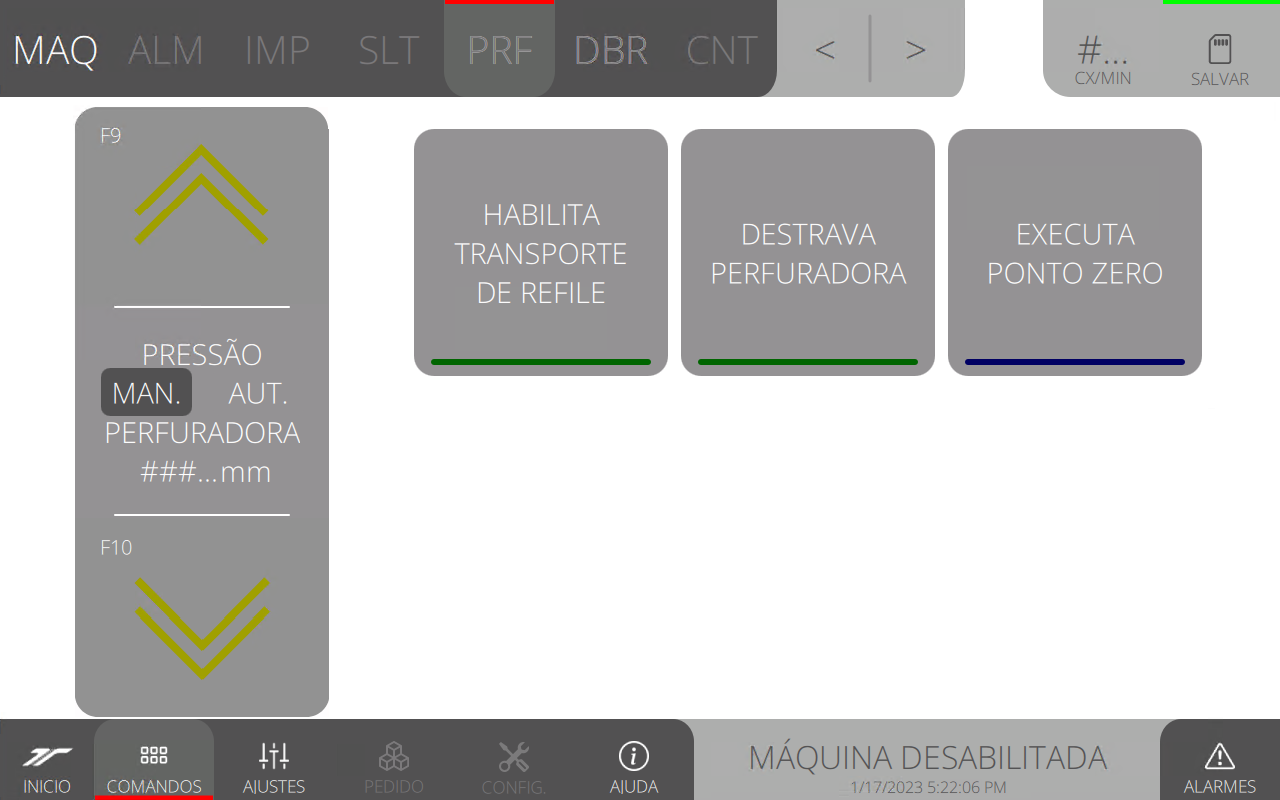
\includegraphics[width=576px,height=360px]{src/imagesFlexo/06-drilling/commands/e-Tela-Principal.png}
\end{figure}
\vspace*{\fill}

\newpage
\thispagestyle{fancy}
\vspace*{40 pt}
\subsubsection{\small{Ajuste pressão porta manta}}\label{telaComandoPerfuradoraAjustePressaoPortaManta}
\vspace*{\fill}
\begin{figure}[h]
  \centering
  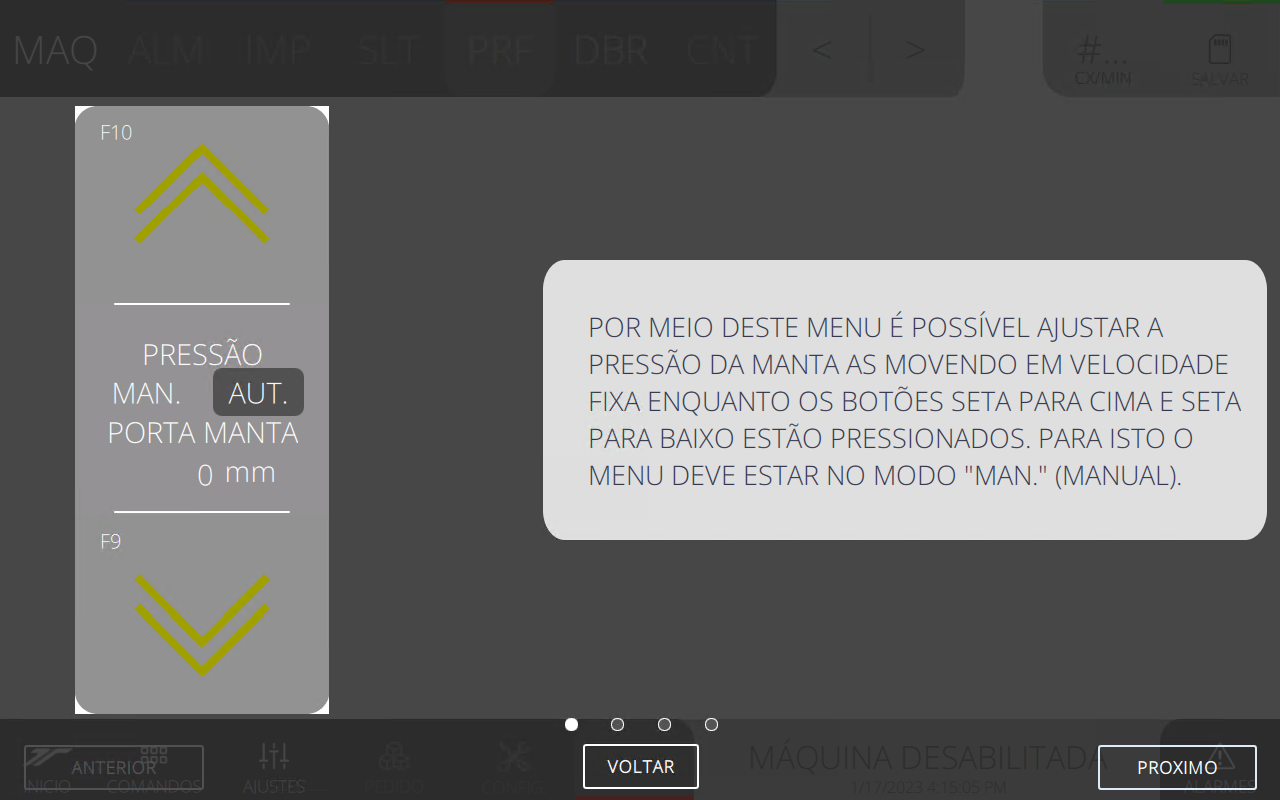
\includegraphics[width=576px,height=360px]{src/imagesFlexo/06-drilling/commands/e-1.png}
\end{figure}
\vspace*{\fill}

\newpage
\thispagestyle{fancy}
\vspace*{40 pt}
\subsubsection{\small{Executa ponto zero}}\label{telaComandoPerfuradoraExecutaPontoZero}
\vspace*{\fill}
\begin{figure}[h]
  \centering
  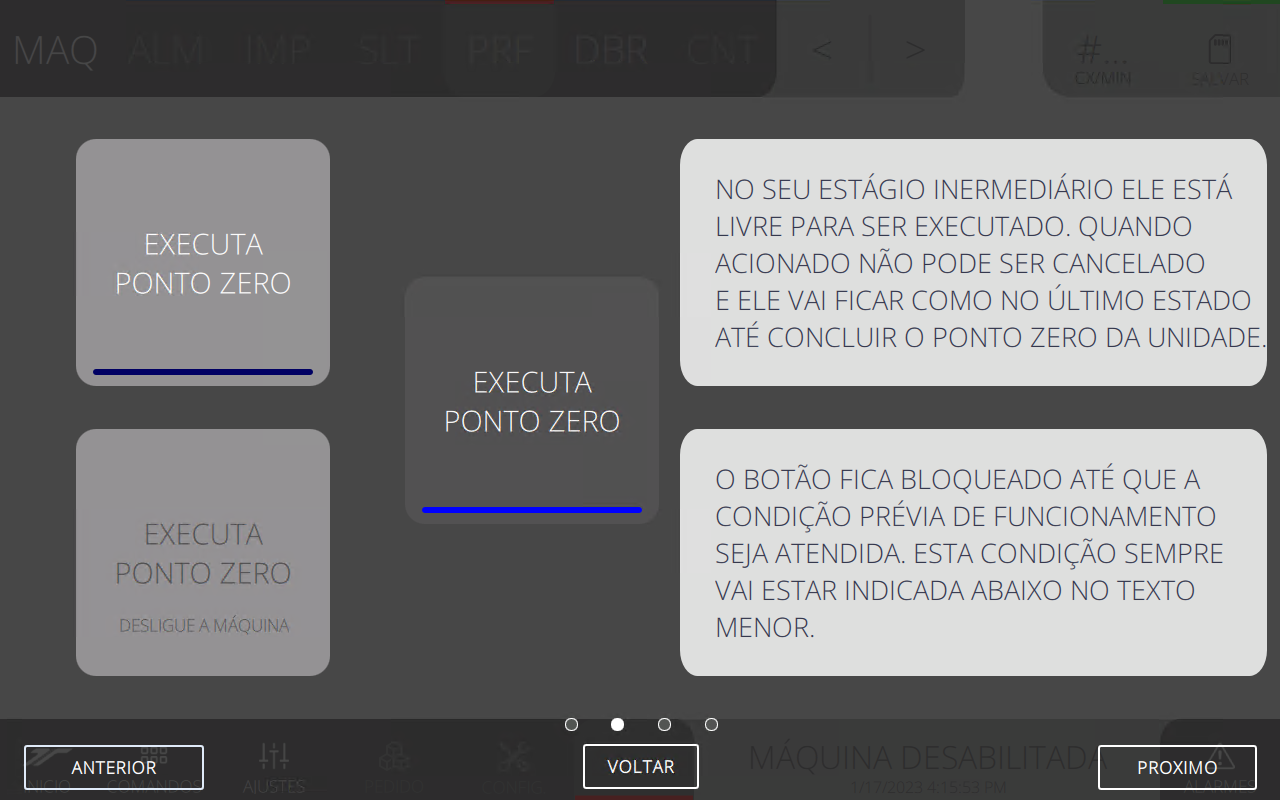
\includegraphics[width=576px,height=360px]{src/imagesFlexo/06-drilling/commands/e-2.png}
\end{figure}
\vspace*{\fill}

\newpage
\thispagestyle{fancy}
\vspace*{40 pt}
\subsubsection{\small{Habilita transporte de refile}}\label{telaComandoPerfuradoraHabilitaTransporteRefile}
\vspace*{\fill}
\begin{figure}[h]
  \centering
  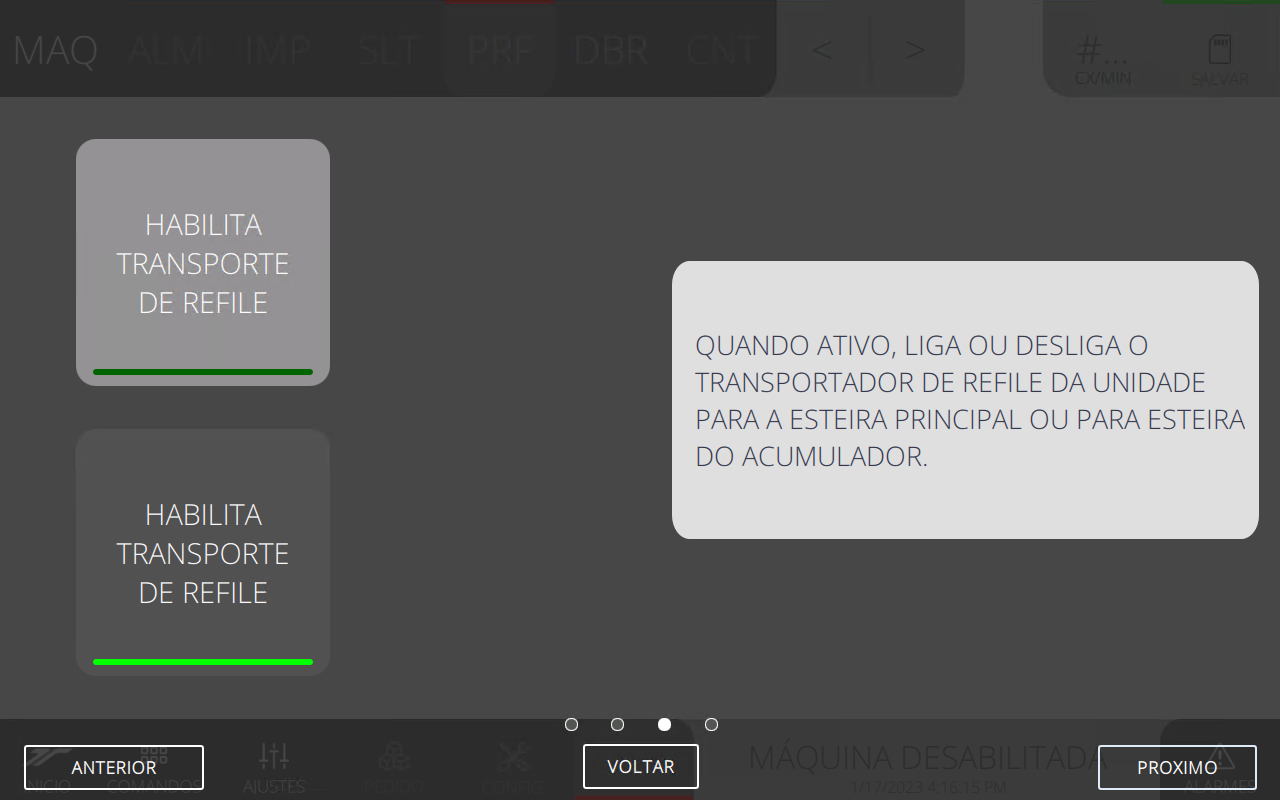
\includegraphics[width=576px,height=360px]{src/imagesFlexo/06-drilling/commands/e-3.png}
\end{figure}
\vspace*{\fill}

\newpage
\thispagestyle{fancy}
\vspace*{40 pt}
\subsubsection{\small{Trava perfuradora}}\label{telaComandoPerfuradoraTravaPerfuradora}
\vspace*{\fill}
\begin{figure}[h]
  \centering
  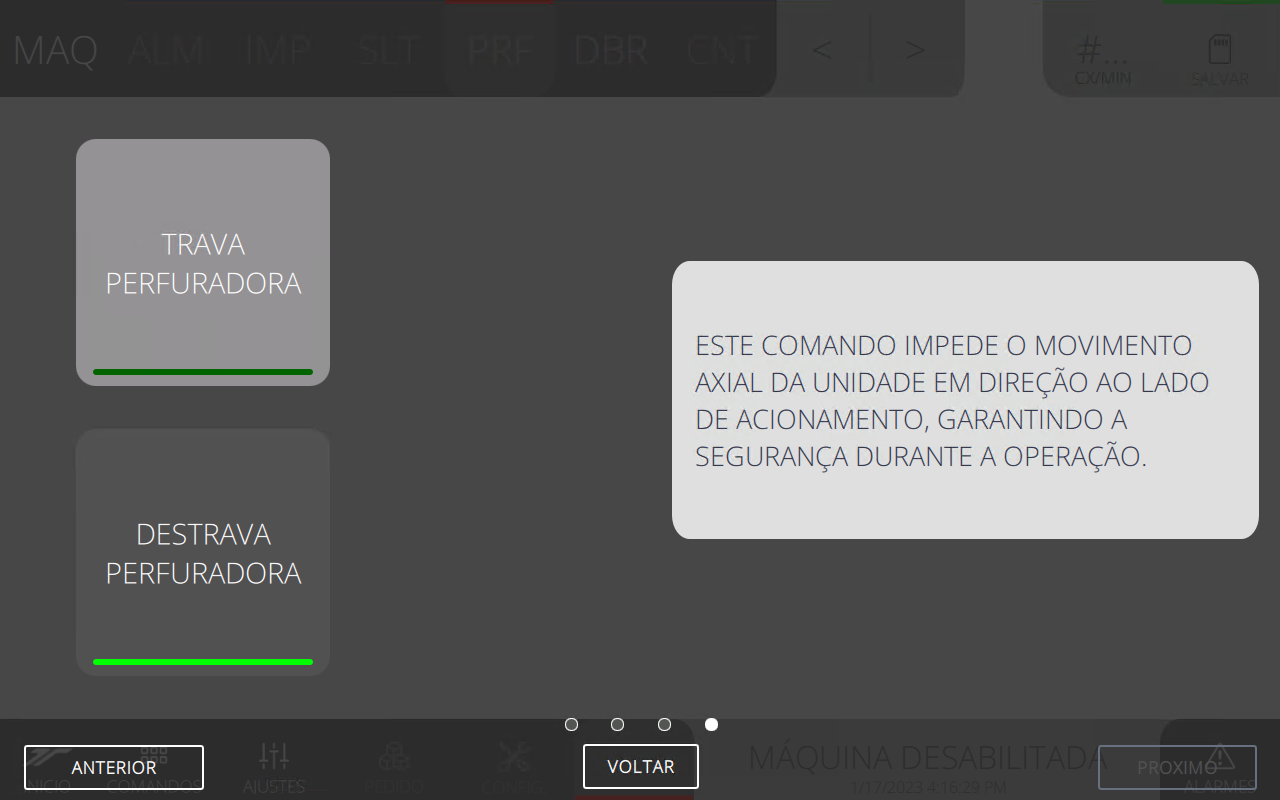
\includegraphics[width=576px,height=360px]{src/imagesFlexo/06-drilling/commands/e-4.png}
\end{figure}
\vspace*{\fill}
